\subsection{Implementación vectorial mediante lista de hijos}
En la implementación vectorial mediante una lista de hijos, cada nodo tiene almacenado una lista de nodos llamados hijos, la cual podemos recorrer para poder consultar sus diferentes hijos (mediante un bucle \texttt{while}).

\begin{figure}[h]
  \begin{center}
    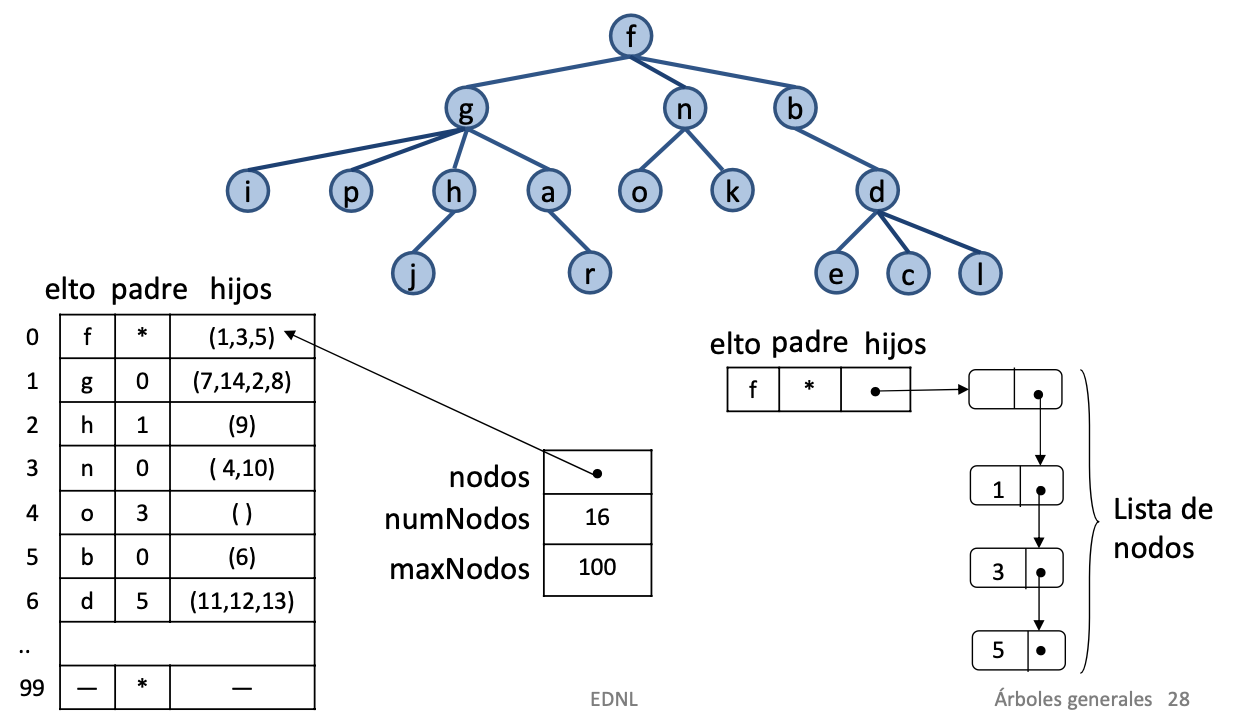
\includegraphics[width=0.75\textwidth]{assets/AgenVec1.png}
  \end{center}
  \caption{Representación de la implementación vectorial mediante lista de hijos.}
\end{figure}

En la parte privada de la implementación de dicho TAD vamos a encontrar el elementos que se almacena, el nodo padre y la lista de los diferentes hijos de cada nodo, todo almacenado en celdas:
\begin{minted}[breaklines]{C++}
template <typename T> class Agen{
  public:
    //Métodos vistos en la especificación del TAD
  private:
    struct celda{
      T elto; //elemento
      nodo padre
      Lista<nodo>hijos;
    };
    celda *nodos; //Vector de nodos
    size_t maxNodos; //Tamaño de vector (árbol)
    size_t numNodos; //Número de nodos en el árbol
};
\end{minted}

